\documentclass[11pt, a4paper]{article} % sets font size and layout

%% required packages %%

\usepackage[margin=2.5cm]{geometry} % margins
\usepackage[utf8]{inputenc} % Umlaute
\usepackage{amsmath,amssymb,physics} % math formulas
\usepackage{graphicx} % graphics
\usepackage{fancyhdr} % header and footer on every page
\usepackage{setspace} % line space
\usepackage{braket}
\usepackage{xcolor}

%% Here the main part of the document begins %%

\begin{document}

%% Some more settings %%

\setlength{\parindent}{0pt} % first line in paragraph will not be indented
\onehalfspacing % 1.5 line spacing

\vspace*{0.1cm}

\begin{center}
	{\Large \textbf{Classical Mechanics}}
    \vspace*{2mm}

    {\Large \textbf{Exemption Exam }}
	\vspace{8mm}

{\Large \textbf{Time: 9:30 am --12:00 pm, Sep. 8th, 2026}}
\vspace*{2mm}

{\Large \textbf{Duration: 150 minutes}}
\vspace*{2mm}

{\Large \textbf{Total Points: 100 points + 6 bonus points}}
\end{center}
\vspace*{8mm}

{\Large \textbf{Instructions:}}
\vspace*{2mm}

{\Large \textbf{This is a closed-book exam; no aids are allowed.}}
\vspace*{2mm}

{\Large \textbf{The exam has 11 pages, including this instruction page.}}
\vspace*{2mm}

{\Large \textbf{Provide relevant mathematical steps.}}
\vspace*{2mm}

{\Large \textbf{All answers must be in English.}}
\vspace*{2mm}

{\Large \textbf{Do not open the booklet before the exam begins.}}
\vspace{5cm}

\begin{center}
{\Large \textbf{Student Name:} \underline{\hspace{4cm}}}
\vspace*{8mm}

{\Large \textbf{Student ID:} \underline{\hspace{4cm}}}
\vspace*{2mm}
\end{center}

\newpage

\section*{Problem 1 [$5 + 5$ points]}
\begin{enumerate}
  \item[(1)] Write down Newton's second law, the Euler--Lagrange equation, and Hamilton's equations of motion for generalized coordinates.

  \item[(2)] Derive the Euler--Lagrange equation from Hamilton's principle. For a system with action
  \[
  S[q]=\int_{t_1}^{t_2} L(q,\dot{q},t)\,dt,
  \]
  show that the condition \(\delta S=0\) for fixed-endpoint variations \(\delta q(t_1)=\delta q(t_2)=0\) leads to the Euler--Lagrange equation.
\end{enumerate}

\newpage

\section*{Problem 2 [$10$ points]}
Use the type-1 generating function
\[
F_1(q,Q)=\frac{1}{2}m\omega q^2\cot Q
\]
for the harmonic oscillator with Hamiltonian
\[
H(q,p)=\frac{p^2}{2m}+\frac{1}{2}m\omega^2q^2
\]
to find the transformed Hamiltonian \(K(Q,P)\). Assume \(F_1\) is time-independent.

\newpage

\section*{Problem 3 [$10$ points]}
A bead of mass \(m\) slides without friction on a circular hoop of radius \(R\). The hoop lies in a vertical plane, but is rotated about its vertical diameter. Suppose the angular velocity \(\Omega(t)\) of the hoop is rapidly modulated in time:
\[
\Omega(t)=\Omega_0+\epsilon \cos(\omega t),
\]
where \(\epsilon\) is small, \(\epsilon/\omega\ll 1\), and \(\omega\) is very large compared with the natural gravitational frequency \(\sqrt{g/R}\). Let \(\theta\) be the angle of the bead measured from the top of the hoop, so that \(\theta=0\) corresponds to the bead being at the unstable upper point when the hoop is not rotating.

Using the Lagrangian formalism, derive the equation of motion for \(\theta(t)\). Within the small-angle approximation about \(\theta=0\), linearize the equation of motion. Keeping only terms up to first order in \(\epsilon\), determine whether the coefficient multiplying \(\theta\) can become negative for small \(\epsilon\). Based on this, discuss whether the rapid modulation stabilizes or destabilizes the top equilibrium.

\begin{figure}[h]
    \centering
    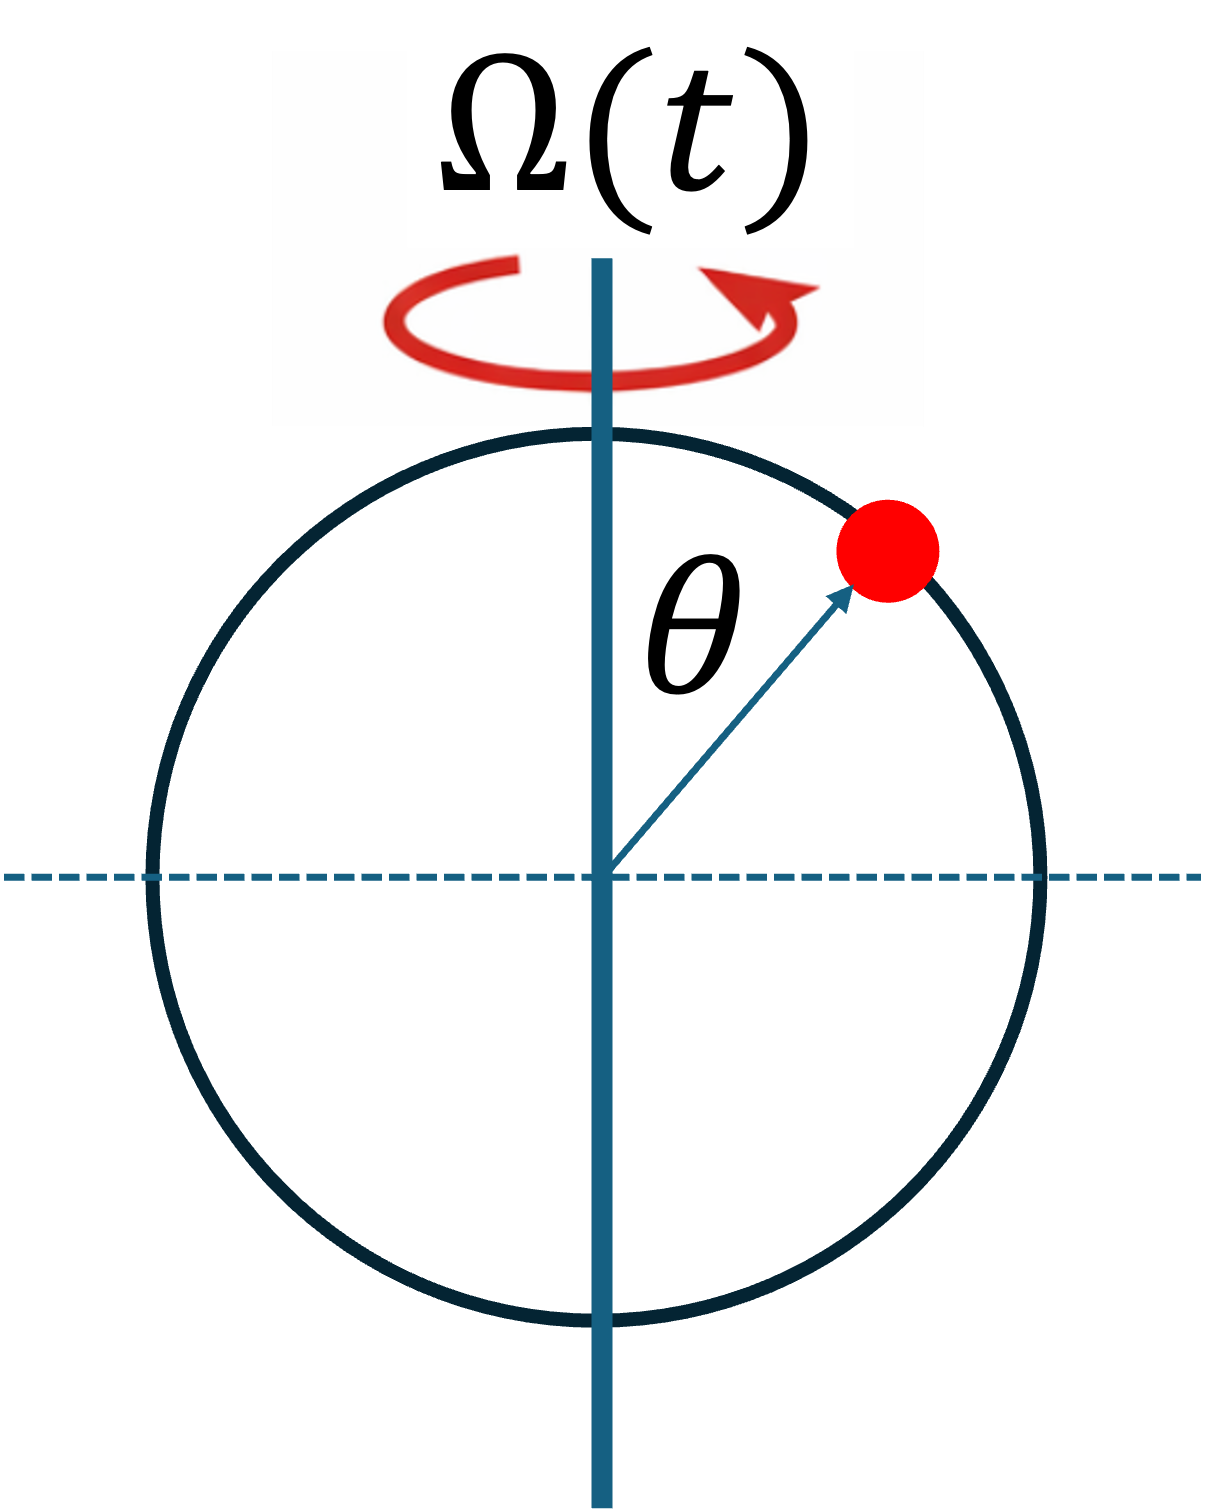
\includegraphics[width=0.3\textwidth]{P3.png}
    \label{P3}
\end{figure}

\newpage

\section*{Problem 4 [$10$ points]}
A block of mass \(m\) is released from rest on a frictionless wedge of mass \(M\) and angle of inclination \(\alpha\). The wedge rests on a frictionless horizontal surface. What is the horizontal acceleration of the wedge of mass \(M\)?

\begin{figure}[h]
    \centering
    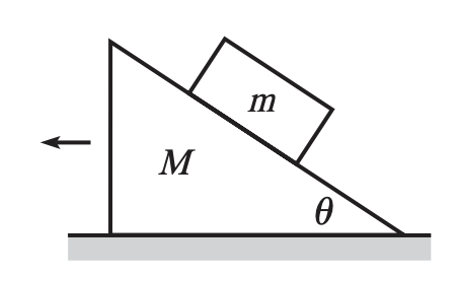
\includegraphics[width=0.6\textwidth]{P4.png}
    \label{P4}
\end{figure}

\newpage

\section*{Problem 5 [$5 + 5$ points]}
A particle of mass \(m\) moves in one dimension with Lagrangian
\[
    L(q,\dot{q})=\frac{1}{2}m\dot{q}^2+A(q)\dot{q}-V(q),
\]
where \(A(q)\) and \(V(q)\) are given functions.

\begin{enumerate}
\item[(1)] Find the canonical momentum \(p\) conjugate to \(q\).

\item[(2)] Find the Hamiltonian \(H(q,p)\).
\end{enumerate}

\newpage

\section*{Problem 6 [$6 + 10$ points]}
\begin{enumerate}
\item[(1)] What conditions must the small constants \(a\), \(b\), \(c\), \(d\), \(e\), and \(f\) satisfy in order that the transformation
\[
    q= Q+ aQ^2+2bQP + cP^2
\]
\[
   p=P+dQ^2+2eQP+fP^2
\]
be canonical to first order in the small constants?

\item[(2)] The Hamiltonian for a slightly anharmonic oscillator is
\[
   H=\frac{p^2}{2m} + \frac{1}{2}m\omega^2q^2 + \beta q^3,
\]
where \(\beta\) is small. Perform a canonical transformation of the type given in part (1) and choose the constants so that the transformed Hamiltonian \(H'\) contains no cubic anharmonic term to first order in the small quantities. Thus,
\[
   H'=\frac{P^2}{2m} + \frac{1}{2}m\omega^2Q^2 + \cdots .
\]
Write down the transformation rules between \((q,p)\) and \((Q,P)\).
\end{enumerate}

\newpage

\section*{Problem 7 [$12$ points]}
A mass \(m\) is attached to one end of a massless spring of natural length \(l_0\) and spring constant \(k\). The other end of the spring is attached to a pivot point that oscillates vertically according to
\[
Y(t)=A\cos(\Omega t).
\]
Let \(Y(t)\) be measured upward. The mass moves in a vertical plane. Let \(r\) be the instantaneous length of the spring, and let \(\theta\) be the angle the spring makes with the downward vertical direction. This is a spring pendulum whose pivot oscillates vertically. Construct the Lagrangian for the system and derive the equations of motion for \(r(t)\) and \(\theta(t)\).

\begin{figure}[h]
    \centering
    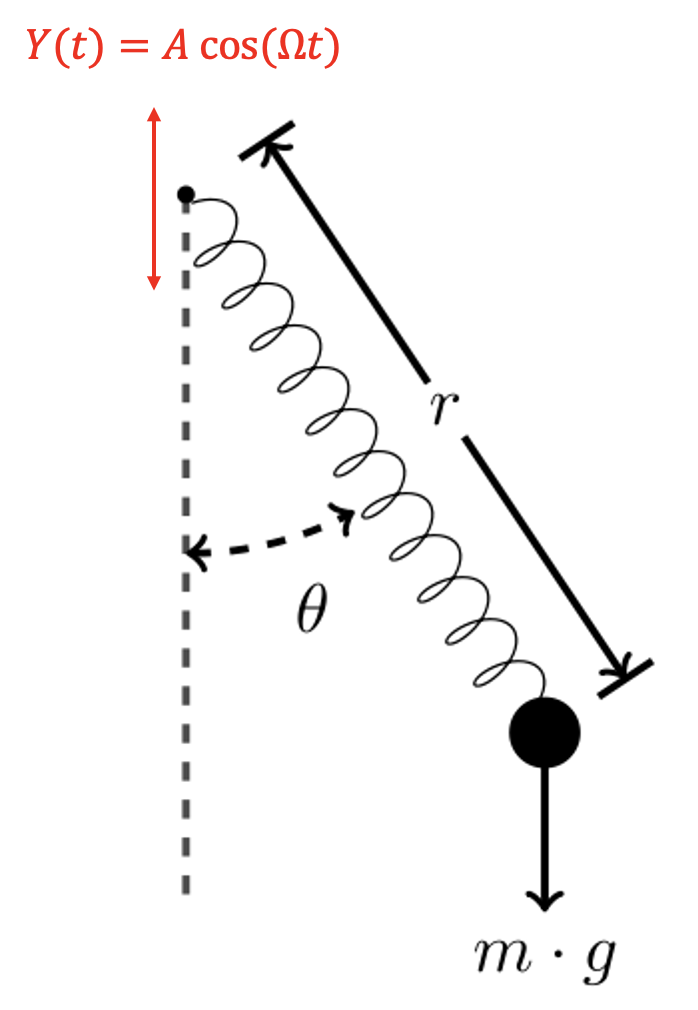
\includegraphics[width=0.4\textwidth]{P7.png}
    \label{P7}
\end{figure}

\newpage

\section*{Problem 8 [$12$ points]}
A satellite of mass \(m\) carrying a crew is initially in a stable circular orbit, Orbit 1, of radius \(R_1\) around a central body of mass \(M\). The crew wishes to transfer the satellite to a larger circular orbit, Orbit 3, with radius \(R_3 = 2R_1\). To achieve this, they perform a maneuver involving two successive impulsive boosts.

First, the satellite performs an initial boost that increases its velocity instantaneously, placing it onto an elliptical transfer orbit, denoted Orbit 2. This transfer orbit has its perigee at radius \(R_1\) and its apogee at radius \(R_3 = 2R_1\).

Next, upon reaching the apogee of the transfer orbit, point \(P'\), the satellite performs a second instantaneous velocity change. This second boost increases the satellite's speed such that it transitions into a final circular orbit of radius \(2R_1\).

\begin{enumerate}
    \item[(1)] Determine the velocity boost factor \(\lambda\) required for the first boost, defined as the ratio of the speed after the boost to the speed before the boost:
    \[
    \lambda = \frac{v_p}{v_1}.
    \]

    \item[(2)] Determine the velocity boost factor \(\lambda'\) required for the second boost, defined as the ratio of the speed after the boost to the speed before the boost:
    \[
    \lambda' = \frac{v_3}{v_{p'}}.
    \]
\end{enumerate}

\textbf{Hint:} The orbit of a satellite is given by
$
r(\phi) = \frac{c}{1 + e\cos \phi}.
$
Here \(e\) is the eccentricity of the orbit and
$
c = \frac{L^2}{GMm^2},
$
where \(L\) is the satellite's angular momentum.

\begin{figure}[h]
    \centering
    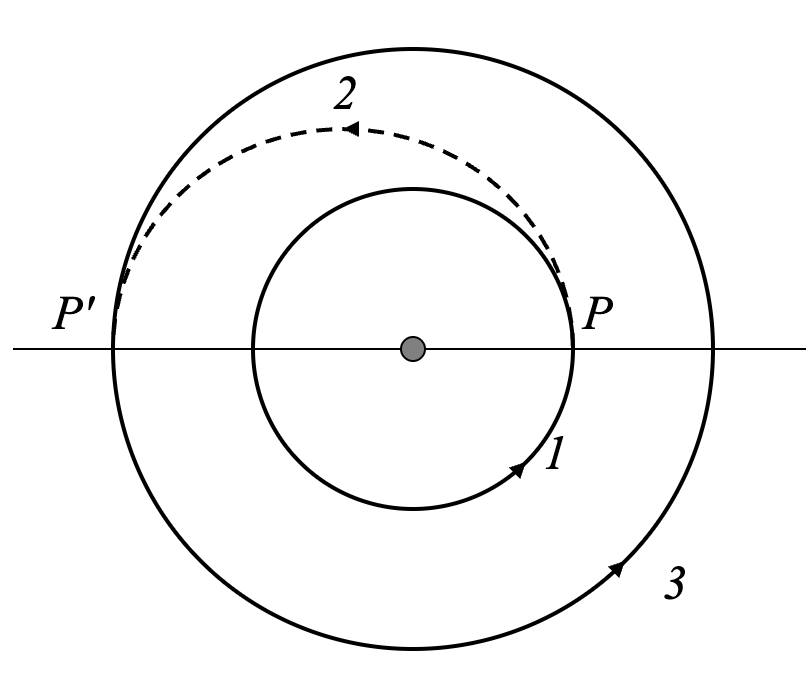
\includegraphics[width=0.3\textwidth]{transfer.png}
    \label{P8}
\end{figure}

\newpage

\section*{Problem 9 [$10$ points]}
The Lagrangian for a particle of mass \(m\) and charge \(e\) moving in a uniform magnetic field pointing in the \(z\)-direction is
\[
L = \frac{1}{2}m\left(\dot{x}^2 + \dot{y}^2  + \dot{z}^2 \right)
+ \frac{eB}{2c}\left(x\dot{y} - y\dot{x}\right).
\]
Show that under the infinitesimal displacement \(x\to x+\varepsilon\), the Lagrangian changes only by a total time derivative. Use Noether's theorem to find the associated conserved quantity.

\newpage

\section*{Bonus Problem [$6$ points]}
The Hamiltonian for a simple harmonic oscillator is
\[
H=\frac{p^2}{2m}+\frac{1}{2}m\omega^2 x^2.
\]
Introduce the complex quantities
\[
a=\sqrt{\frac{m\omega}{2}}\left(x+\frac{i p}{m\omega}\right),
\qquad
a^*=\sqrt{\frac{m\omega}{2}}\left(x-\frac{i p}{m\omega}\right).
\]

\begin{enumerate}
    \item[(a)] Express \(H\) in terms of \(a\) and \(a^*\).

    \item[(b)] Evaluate the Poisson brackets \(\{a,a^*\}\), \(\{a,H\}\), and \(\{a^*,H\}\).
\end{enumerate}

\end{document}

